% !TEX TS-program = pdflatex
% !TEX encoding = UTF-8 Unicode

% This is a simple template for a LaTeX document using the "article" class.
% See "book", "report", "letter" for other types of document.

\documentclass[11pt]{article} % use larger type; default would be 10pt

\usepackage[utf8]{inputenc} % set input encoding (not needed with XeLaTeX)

%%% Examples of Article customizations
% These packages are optional, depending whether you want the features they provide.
% See the LaTeX Companion or other references for full information.

%%% PAGE DIMENSIONS
\usepackage{geometry} % to change the page dimensions
\geometry{a4paper} % or letterpaper (US) or a5paper or....
% \geometry{margin=2in} % for example, change the margins to 2 inches all round
% \geometry{landscape} % set up the page for landscape
%   read geometry.pdf for detailed page layout information

\usepackage{graphicx} % support the \includegraphics command and options
\usepackage[outdir=./]{epstopdf}
% \usepackage[parfill]{parskip} % Activate to begin paragraphs with an empty line rather than an indent

%%% PACKAGES
\usepackage{booktabs} % for much better looking tables
\usepackage{array} % for better arrays (eg matrices) in maths
\usepackage{paralist} % very flexible & customisable lists (eg. enumerate/itemize, etc.)
\usepackage{verbatim} % adds environment for commenting out blocks of text & for better verbatim
\usepackage{subfig} % make it possible to include more than one captioned figure/table in a single float
\usepackage{url}
\usepackage{diagbox}
% These packages are all incorporated in the memoir class to one degree or another...

%%% HEADERS & FOOTERS
\usepackage{fancyhdr} % This should be set AFTER setting up the page geometry
\pagestyle{fancy} % options: empty , plain , fancy
\renewcommand{\headrulewidth}{0pt} % customise the layout...
\lhead{}\chead{}\rhead{}
\lfoot{}\cfoot{\thepage}\rfoot{}

%%% SECTION TITLE APPEARANCE
\usepackage{sectsty}
\allsectionsfont{\sffamily\mdseries\upshape} % (See the fntguide.pdf for font help)
% (This matches ConTeXt defaults)

%%% ToC (table of contents) APPEARANCE
\usepackage[nottoc,notlof,notlot]{tocbibind} % Put the bibliography in the ToC
\usepackage[titles,subfigure]{tocloft} % Alter the style of the Table of Contents
\renewcommand{\cftsecfont}{\rmfamily\mdseries\upshape}
\renewcommand{\cftsecpagefont}{\rmfamily\mdseries\upshape} % No bold!

%%% END Article customizations

%%% The "real" document content comes below...

\title{CLP Lab 1 Report}
\author{Albert Aparicio Isarn\\
	\url{albert.aparicio.isarn@alu-etsetb.upc.edu}
	\and 
	Héctor Esteban\\
	\url{hect.esteban@gmail.com}}
\date{} % Activate to display a given date or no date (if empty),
         % otherwise the current date is printed 

\begin{document}
\maketitle

\section[Parte 1 - ROC]{Análisis de curvas ROC}

En las tablas \ref{tab:p1:linear} y \ref{tab:p1:quadratic} se muestran las probabilidades de error para los clasificadores Lineal y Cuadrático, respectivamente.
\begin{table}[h]
	\begin{center}
		\begin{tabular}{| l | c | c | c | c |}
			\hline
			\diagbox[width=8em]{\textbf{Clase}}{\textbf{SNR}} & \textbf{3 dB} & \textbf{0 dB} & \textbf{-3 dB} & {-10 dB} \\
			\hline
			\textbf{Clase 1} & $ 5 \cdot 10^{-3} $ & $ 0.042 $ & $ 0.107$ & 0.3 \\
			\hline
			\textbf{Clase 2} & $ 8 \cdot 10^{-3} $ & $ 0.034 $ & $ 0.106 $ & 0.31 	\\
			\hline
		\end{tabular}
		\caption{Probabilidades de error para el clasificador Lineal (LC)}
		\label{tab:p1:linear}
	\end{center}
\end{table}

\begin{table}[h]
	\begin{center}
		\begin{tabular}{| l | c | c | c | c |}
			\hline
			\diagbox[width=8em]{\textbf{Clase}}{\textbf{SNR}} & \textbf{3 dB} & \textbf{0 dB} & \textbf{-3 dB} & {-10 dB} \\
			\hline
			\textbf{Clase 1} & $ 7 \cdot 10^{-3} $ & $ 0.041 $ & $ 0.114$ & 0.292 \\
			\hline
			\textbf{Clase 2} & $ 3 \cdot 10^{-3} $ & $ 0.036 $ & $ 0.118 $ & 0.306 	\\
			\hline
		\end{tabular}
		\caption{Probabilidades de error para el clasificador Cuadrático (QC)}
		\label{tab:p1:quadratic}
	\end{center}
\end{table}

En las figuras \ref{fig:p1:roc:-3} y \ref{fig:p1:roc:-10} se muestran las curvas ROC para los casos de -3 y -10 dB, respectivamente.

\begin{figure}[h]
	\centering
	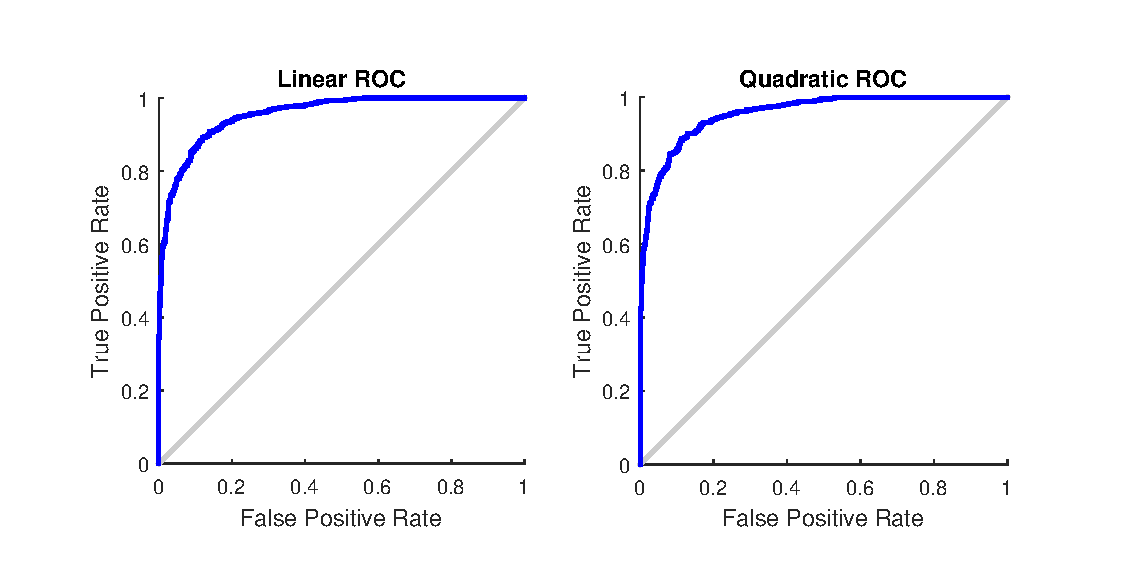
\includegraphics[width=\textwidth]{ROC_-3.eps}
	\caption[]{\small Gráficos de los tests de gausianidad de las cuatro distribuciones sintéticas.} 
	\label{fig:p1:roc:-3}
\end{figure}

\section[Parte 2 - Autovalor]{Autovalores de matriz de covarianza y
	forma de los clusters}

\end{document}
